\chapter*{Data Model}
Persistent data will be stored in a relational database. This section discusses the relational database model supporting DERP.

\section*{Overview}
\begin{center}
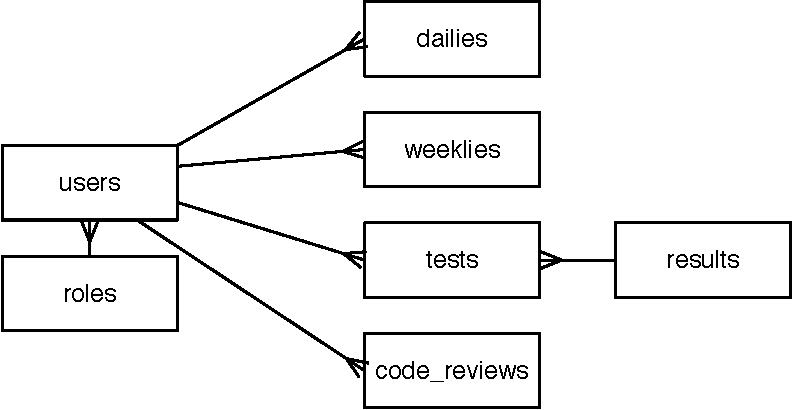
\includegraphics[width=0.8\textwidth]{./erd.pdf}
\end{center}

Each of the major entities (users, dailies, weeklies, and tests) tracked by DERP have an associated table. Users may belong to a limited set of roles and the roles are enumerated by the roles table. Tests have a current status, the valid statuses are enumerated in the results table.

\section*{Table Definitions}
\subsection*{users}
\begin{tabular}{l|l|l}
\hline
user\_pk & integer & primary key for user records \\
github\_username & varchar(128) & username on GitHub \\
duck\_id & varchar(128) & UO username (to correlate with Canvas) \\
email & varchar(128) & preferred email address \\
repo & varchar(256) & https URL for developer's repo \\
role\_fk & integer & foreign key to roles.role\_pk \\
\hline
\end{tabular}

\subsection*{roles}
\begin{tabular}{l|l|l}
\hline
role\_pk & integer & primary key for role records \\
role\_name & varchar(128) & string representation \\
\hline
\end{tabular}

Roles that are expected in the initial version are `new user', `developer', and `manager'.

\subsection*{dailies}
\begin{tabular}{l|l|l}
\hline
daily\_pk & integer & primary key for daily records \\
user\_fk & integer & foreign key to users.user\_pk \\
create\_dt & timestamp & time the daily was created \\
message & varchar(500) & daily message text \\
\hline
\end{tabular}

\subsection*{weeklies}
\begin{tabular}{l|l|l}
\hline
weekly\_pk & integer & primary key for weekly records \\
user\_fk & integer & foreign key to users.user\_pk \\
create\_dt & timestamp & time the weekly was created \\
accomplishments & text & what was accomplished \\
next\_steps & text & what will be worked on next \\
challenges & text & anticipated challenges \\
comments & text & open area for comments \\
\hline
\end{tabular}

\subsection*{code\_reviews}
\begin{tabular}{l|l|l}
\hline
review\_pk & integer & primary key for weekly records \\
reviewer\_fk & integer & foreign key to users.user\_pk \\
reviewee\_fk & integer & foreign key to users.user\_pk \\
released & boolean & has been released for the reviewee \\
assigned\_dt & timestamp & date the review assignment was made \\
review\_dt & timestamp & date the review was submitted \\
comments & text & review text \\
\hline
\end{tabular}

\subsection*{tests}
\begin{tabular}{l|l|l}
\hline
test\_pk & integer & primary key for test records \\
user\_fk & integer & foreign key to users.user\_pk \\
create\_dt & timestamp & time the test was created \\
result\_fk & integer & foreign key to results.result\_pk \\
complete\_dt & timestamp & time the test finished \\
message & text & test output \\
\hline
\end{tabular}

\subsection*{results}
\begin{tabular}{l|l|l}
\hline
result\_pk & integer & primary key for result records \\
result\_name & varchar(128) & string representation \\
\hline
\end{tabular}

The results table is poorly named. This table enumerates the states a test record may be in. Results that are expected in the initial version are `in queue', `cancelled', `running', `passed', `failed', and `partial'.
